\documentclass[9pt]{beamer}

% Beamer style
%\usetheme[secheader]{Madrid}
% \usetheme{CambridgeUS}
\useoutertheme{infolines}
\usecolortheme[rgb={0.65,0.15,0.25}]{structure}
% \usefonttheme[onlymath]{serif}
\beamertemplatenavigationsymbolsempty
%\AtBeginSubsection

% Packages
%\usepackage[french]{babel}
\usepackage[latin1]{inputenc}
\usepackage{color}
\usepackage{xspace}
\usepackage{dsfont, stmaryrd}
\usepackage{amsmath, amsfonts, amssymb, stmaryrd}
\usepackage{epsfig}
\usepackage{tikz}
\usepackage{url}
% \usepackage{ulem}
\usepackage{/home/robin/LATEX/Biblio/astats}
%\usepackage[all]{xy}
\usepackage{graphicx}
\usepackage{xspace}

\input{/home/robin/RECHERCHE/EXPOSES/LATEX/Commands}

% Directory
\newcommand{\ts}{{\theta^{*}}}
\newcommand{\kl}{{(k\ell)}}
\newcommand{\fignet}{/home/robin/Bureau/RECHERCHE/RESEAUX/EXPOSES/FIGURES}
\newcommand{\figtree}{/home/robin/RECHERCHE/BAYES/VBEM-IS/VBEM-IS.git/Data/Tree/Fig}
\newcommand{\figzebra}{/home/robin/RECHERCHE/BAYES/VBEM-IS/VBEM-IS.git/Data/Zebra/Fig}

%====================================================================
%====================================================================

%====================================================================
%====================================================================
\begin{document}
%====================================================================
%====================================================================

%====================================================================
\title[SBM: Beyond variational inference]{Stochastic blockmodels: Beyond variational inference}

\author[S. Robin]{S. Robin \\ ~ \\
joint work with C. Matias and S. Donnet \\ ~}

\institute[]{INRA / AgroParisTech / univ. Paris-Saclay}

\date[Bordeaux, Apr. 2019]{S�minaire de Statistique Bordelais, Avril 2019}

%====================================================================
%====================================================================
\maketitle
%====================================================================

%====================================================================
%====================================================================
\section*{Introduction}
%====================================================================
\frame{\frametitle{Stochastic block model} 

  \paragraph{SBM.} Very popular tool for network analysis \refer{HoL79,NoS01}
  
  \bigskip \bigskip \pause
  \paragraph{Principle.} Model-based graph clustering:
  \begin{itemize}
   \item Nodes belong to unobserved groups
   \item Interactions between nodes depend on node's membership
  \end{itemize}

  \bigskip \bigskip \pause
  \paragraph{Statistical inference.} 
  \begin{itemize}
   \item Intricate network-shaped dependency structure
   \item Difficult statistical inference (intractable MLE, no EM)
   \item Most often: resort to (computationally efficient) variational approximations, with few statistical guaranties
  \end{itemize}
  \ra Can we build upon variational inference to make statistical inference?
}

%====================================================================
%====================================================================
\section{Variational inference for the stochastic block model}
\subsection*{Model}
\frame{\frametitle{Outline} \tableofcontents}
\frame{\frametitle{Outline} \tableofcontents[currentsection]}
%====================================================================
\frame{\frametitle{Binary SBM} 

  \paragraph{Data at hand.}
  \begin{itemize}
   \item $Y = (Y_{ij})_{1 \leq i, j, \leq n}= n \times n$ matrix: 
   $$
   Y_{ij} =  \text{link between individual $i$ and $j$}
   $$
  \end{itemize}
  
  \bigskip \pause
  \paragraph{Model.} $K$ groups
  \begin{itemize}
  \item $(Z_i)_{1 \leq i \leq n} = $ iid node memberships (with proportion $\pi$)
  \item $(Y_{ij})_{1 \leq i, j \leq n} =$ conditionally independent : $P(Y_{ij} = 1 \mid Z_i, Z_j ) = p_{k\ell}$
  \end{itemize}

  $$
  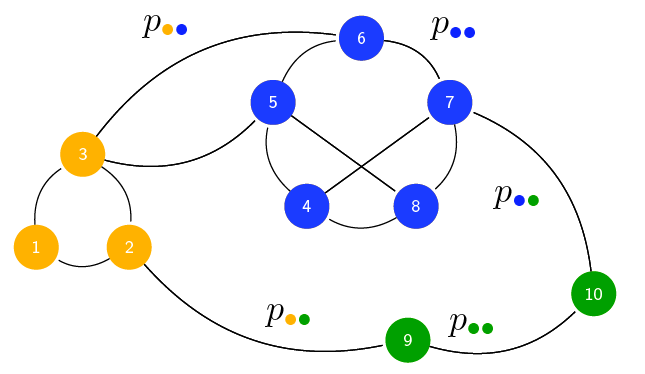
\includegraphics[width=.4\textwidth]{../FIGURES/SBM-CMatias}
  $$
}

%====================================================================
\frame{\frametitle{General SBM} 

  \paragraph{Data at hand.}
  \begin{itemize}
   \item $Y = (Y_{ij})_{1 \leq i, j, \leq n}= n \times n$ matrix: 
   $$
   Y_{ij} =  \text{interaction strength between individual $i$ and $j$}
   $$
   \item $x_{ij} =$ vector of covariates for the pair $(i, j)$
  \end{itemize}
  
  \bigskip \bigskip \pause
  \paragraph{Model.} $K$ groups
  \begin{itemize}
  \item Same $(Z_i)$ as before
  \item $(Y_{ij})_{1 \leq i, j \leq n} =$ conditionally independent : $Y_{ij} \mid Z_i, Z_j \sim f(\cdot; \gamma_{Z_i Z_j}, x_{ij}) $
  \end{itemize}
  \ra Node clusters are independent from covariates' effect

  \bigskip \bigskip \pause
  \paragraph{Example.} Poisson distributed edges \refer{MRV10}:
  \begin{align*}
    (Y_{ij} \mid Z_i=k, Z_j = \ell) & \sim \Pcal\left(e^{\alpha_{kl} + x_{ij}^\intercal \beta}\right) \\
  \gamma_{kl} & = (\alpha_{kl}, \beta), 
  \qquad \qquad \theta = (\pi, \alpha, \beta)
  \end{align*}
}

%====================================================================
\frame{\frametitle{Example: Tree network}

  \hspace{-.025\textwidth}
  \begin{tabular}{ll}
   \begin{tabular}{p{.35\textwidth}}
    \paragraph{From \refer{VPD08}.} 
    $n = 51$ tree species 

    \bigskip
    $Y_{ij} = $ number of shared fungal parasites 

    \bigskip
    3 covariates (distances): \\
    taxonomy, geography, genetics 

    \bigskip
    \paragraph{Poisson model:} \\
    $(Y_{ij} \mid Z_i=k, Z_j=\ell)$ \\ \smallskip
    $\qquad \sim \Pcal\left(e^{\alpha_{k\ell} + x_{ji}^\intercal \beta}\right)$ 
   \end{tabular}
   &
   \hspace{-.05\textwidth}
   \begin{tabular}{c|c}
    \includegraphics[width=.25\textwidth]{\figtree/Tree-all-V10-M5000-net} & 
    \includegraphics[width=.25\textwidth]{../FIGURES/FigVBEM-IS-Tree-TaxonomicDistance} \\
    Interactions & Taxonomic dist. \\ \hline
    \includegraphics[width=.25\textwidth]{../FIGURES/FigVBEM-IS-Tree-GeographicDistance} & 
    \includegraphics[width=.25\textwidth]{../FIGURES/FigVBEM-IS-Tree-GeneticDistance}  \\
    Geographic dist. & Genetic dist.
   \end{tabular}
  \end{tabular}

}

%====================================================================
\frame{\frametitle{Inference} 

  \paragraph{Observed likelihood.}
  $$
  \log p_\theta(Y) = \log \left(\sum_{z \in \{1 \dots K\}^n} P_\pi(Z=z) p_\gamma(Y \mid Z = z) \right)
  $$

  \bigskip \pause
  \paragraph{Complete likelihood.} Denoting $Z_{ik} = \Ibb\{Z_i = k\}$, 
  \begin{align*}
  \log p_\theta(Y, Z) 
    & = \log p_\pi(Z) p_\gamma(Y \mid Z) \\
    \\
    & = \sum_i \emphase{Z_{ik}} \log \pi_k + \sum_{i < j} \sum_{k, \ell} \emphase{Z_{ik} Z_{j\ell}} \log f(Y_{ij}; \gamma_{k\ell}, x_{ij})
  \end{align*}
  \ra EM requires to evaluate $P_\theta(Z_i = k \mid Y)$ and $P_\theta(Z_i = k, Z_j = \ell \mid Y)$.

  \bigskip \bigskip \pause
  \paragraph{GLM framework:} $f \in$ exponential family
  $$
  \log f(Y_{ij}; \gamma_{kl}, x_{ij}) = (\eta_{ij}^{k\ell})^\intercal t(Y_{ij}) - a(Y_{ij}) - b(\eta_{ij}^{k\ell}), 
  \qquad \qquad 
  \eta_{ij}^{k\ell} = \alpha_{kl} + \emphase{x_{ij}^\intercal \beta}
%   \qquad \gamma_{kl} = (\alpha_{kl}, \beta), 
%   \quad \theta = (\pi, \alpha, \beta)
  $$
  \ra M-step $\simeq$ GLM regression
}

%====================================================================
\subsection*{Inference}
%====================================================================
\frame{\frametitle{Inference} 

  \paragraph{Maximum likelihood inference via EM:} requires to evaluate $p(Z \mid Y)$
  
  \bigskip \bigskip 
  \begin{overprint}
  \onslide<1> \paragraph{Graphical model point of view.} $p(Z)$
  \onslide<2> \paragraph{Graphical model point of view.} $p(Z) p(Y_{12} \mid Z_1, Z_2)$
  \onslide<3> \paragraph{Graphical model point of view.} $p(Z) p(Y \mid Z)$
  \onslide<4> \paragraph{Graphical model point of view.} Moralization
  \onslide<5> \paragraph{Graphical model point of view.} $p(Z \mid Y)$: no factorization
  \end{overprint}
  ~\\ ~\
    
  \begin{overprint}
  \onslide<1>
  \begin{centering}
    \begin{tikzpicture}
  \node[hidden] (Z1) at (0, \edgeunit) {$Z_1$};
  \node[hidden] (Z2) at (\edgeunit, \edgeunit) {$Z_2$};
  \node[hidden] (Z3) at (0, 0) {$Z_3$};
  \node[hidden] (Z4) at (\edgeunit, 0) {$Z_4$};

  \node[empty] (Y12) at (.5*\edgeunit, 1.75*\edgeunit) {$Y_{12}$};
  \node[empty] (Y13) at (-.75*\edgeunit, .5*\edgeunit) {$Y_{13}$};
  \node[empty] (Y14) at (1.75*\edgeunit, 1.75*\edgeunit) {$Y_{14}$};
  \node[empty] (Y23) at (-.75*\edgeunit, 1.75*\edgeunit) {$Y_{23}$};
  \node[empty] (Y24) at (1.75*\edgeunit, .5*\edgeunit) {$Y_{24}$};
  \node[empty] (Y34) at (.5*\edgeunit, -.75*\edgeunit) {$Y_{34}$};
  
%   \draw[arrow] (Z1) to (Y12);  \draw[arrow] (Z2) to (Y12);
%   \draw[arrow] (Z1) to (Y13);  \draw[arrow] (Z3) to (Y13);
%   \draw[arrow] (Z1) to (Y14);  \draw[arrow] (Z4) to (Y14);
%   \draw[arrow] (Z2) to (Y23);  \draw[arrow] (Z3) to (Y23);
%   \draw[arrow] (Z2) to (Y24);  \draw[arrow] (Z4) to (Y24);
%   \draw[arrow] (Z3) to (Y34);  \draw[arrow] (Z4) to (Y34);
  \end{tikzpicture}

 
  \end{centering}
  \onslide<2>
  \begin{centering}
    \begin{tikzpicture}
  \node[hidden] (Z1) at (0, \edgeunit) {$Z_1$};
  \node[hidden] (Z2) at (\edgeunit, \edgeunit) {$Z_2$};
  \node[hidden] (Z3) at (0, 0) {$Z_3$};
  \node[hidden] (Z4) at (\edgeunit, 0) {$Z_4$};

  \node[observed] (Y12) at (.5*\edgeunit, 1.75*\edgeunit) {$Y_{12}$};
  \node[empty] (Y13) at (-.75*\edgeunit, .5*\edgeunit) {$Y_{13}$};
  \node[empty] (Y14) at (1.75*\edgeunit, 1.75*\edgeunit) {$Y_{14}$};
  \node[empty] (Y23) at (-.75*\edgeunit, 1.75*\edgeunit) {$Y_{23}$};
  \node[empty] (Y24) at (1.75*\edgeunit, .5*\edgeunit) {$Y_{24}$};
  \node[empty] (Y34) at (.5*\edgeunit, -.75*\edgeunit) {$Y_{34}$};
  
  \draw[arrow] (Z1) to (Y12); \draw[arrow] (Z2) to (Y12);
  \end{tikzpicture}

 
  \end{centering}
  \onslide<3>
  \begin{centering}
    \begin{tikzpicture}
  \node[hidden] (Z1) at (0, \edgeunit) {$Z_1$};
  \node[hidden] (Z2) at (\edgeunit, \edgeunit) {$Z_2$};
  \node[hidden] (Z3) at (0, 0) {$Z_3$};
  \node[hidden] (Z4) at (\edgeunit, 0) {$Z_4$};

  \node[observed] (Y12) at (.5*\edgeunit, 1.75*\edgeunit) {$Y_{12}$};
  \node[observed] (Y13) at (-.75*\edgeunit, .5*\edgeunit) {$Y_{13}$};
  \node[observed] (Y14) at (1.75*\edgeunit, 1.75*\edgeunit) {$Y_{14}$};
  \node[observed] (Y23) at (-.75*\edgeunit, 1.75*\edgeunit) {$Y_{23}$};
  \node[observed] (Y24) at (1.75*\edgeunit, .5*\edgeunit) {$Y_{24}$};
  \node[observed] (Y34) at (.5*\edgeunit, -.75*\edgeunit) {$Y_{34}$};
  
  \draw[arrow] (Z1) to (Y12);  \draw[arrow] (Z2) to (Y12);
  \draw[arrow] (Z1) to (Y13);  \draw[arrow] (Z3) to (Y13);
  \draw[arrow] (Z1) to (Y14);  \draw[arrow] (Z4) to (Y14);
  \draw[arrow] (Z2) to (Y23);  \draw[arrow] (Z3) to (Y23);
  \draw[arrow] (Z2) to (Y24);  \draw[arrow] (Z4) to (Y24);
  \draw[arrow] (Z3) to (Y34);  \draw[arrow] (Z4) to (Y34);
  \end{tikzpicture}

 
  \end{centering}
  \onslide<4>
  \begin{centering}
    \begin{tikzpicture}
  \node[hidden] (Z1) at (0, \edgeunit) {$Z_1$};
  \node[hidden] (Z2) at (\edgeunit, \edgeunit) {$Z_2$};
  \node[hidden] (Z3) at (0, 0) {$Z_3$};
  \node[hidden] (Z4) at (\edgeunit, 0) {$Z_4$};

  \node[observed] (Y12) at (.5*\edgeunit, 1.75*\edgeunit) {$Y_{12}$};
  \node[observed] (Y13) at (-.75*\edgeunit, .5*\edgeunit) {$Y_{13}$};
  \node[observed] (Y14) at (1.75*\edgeunit, 1.75*\edgeunit) {$Y_{14}$};
  \node[observed] (Y23) at (-.75*\edgeunit, 1.75*\edgeunit) {$Y_{23}$};
  \node[observed] (Y24) at (1.75*\edgeunit, .5*\edgeunit) {$Y_{24}$};
  \node[observed] (Y34) at (.5*\edgeunit, -.75*\edgeunit) {$Y_{34}$};
  
  \draw[lightarrow] (Z1) to (Y12);  \draw[lightarrow] (Z2) to (Y12);
  \draw[lightarrow] (Z1) to (Y13);  \draw[lightarrow] (Z3) to (Y13);
  \draw[lightarrow] (Z1) to (Y14);  \draw[lightarrow] (Z4) to (Y14);
  \draw[lightarrow] (Z2) to (Y23);  \draw[lightarrow] (Z3) to (Y23);
  \draw[lightarrow] (Z2) to (Y24);  \draw[lightarrow] (Z4) to (Y24);
  \draw[lightarrow] (Z3) to (Y34);  \draw[lightarrow] (Z4) to (Y34);
  
  \draw[dashededge] (Z1) to (Z2);  \draw[dashededge] (Z1) to (Z3);
  \draw[dashededge] (Z1) to (Z4);  \draw[dashededge] (Z2) to (Z3);
  \draw[dashededge] (Z2) to (Z4);  \draw[dashededge] (Z3) to (Z4);
  \end{tikzpicture}

 
  \end{centering}
  \onslide<5>
  \begin{centering}
    \begin{tikzpicture}
  \node[hidden] (Z1) at (0, \edgeunit) {$Z_1$};
  \node[hidden] (Z2) at (\edgeunit, \edgeunit) {$Z_2$};
  \node[hidden] (Z3) at (0, 0) {$Z_3$};
  \node[hidden] (Z4) at (\edgeunit, 0) {$Z_4$};

  \node[eliminated] (Y12) at (.5*\edgeunit, 1.75*\edgeunit) {$Y_{12}$};
  \node[eliminated] (Y13) at (-.75*\edgeunit, .5*\edgeunit) {$Y_{13}$};
  \node[eliminated] (Y14) at (1.75*\edgeunit, 1.75*\edgeunit) {$Y_{14}$};
  \node[eliminated] (Y23) at (-.75*\edgeunit, 1.75*\edgeunit) {$Y_{23}$};
  \node[eliminated] (Y24) at (1.75*\edgeunit, .5*\edgeunit) {$Y_{24}$};
  \node[eliminated] (Y34) at (.5*\edgeunit, -.75*\edgeunit) {$Y_{34}$};
  
  \draw[edge] (Z1) to (Z2);  \draw[edge] (Z1) to (Z3);
  \draw[edge] (Z1) to (Z4);  \draw[edge] (Z2) to (Z3);
  \draw[edge] (Z2) to (Z4);  \draw[edge] (Z3) to (Z4);
  \end{tikzpicture}

 
  \end{centering}
  \end{overprint}

}

%====================================================================
\frame{\frametitle{Variational inference} 

  \paragraph{Principle \refer{WaJ08,BKM17}.} Choose
  \begin{itemize}
   \item a divergence measure $D(q \mid\mid p)$
   \item a class of distributions $\Qcal$
  \end{itemize}
  and maximize wrt $\theta$ and $q \in \Qcal$ the lower bound
  $$
  \log p_\theta(Y) - D(q(Z) \mid\mid p_\theta(Z \mid Y)) \leq \log p_\theta(Y)
  $$

  \bigskip \pause
  \paragraph{Popular choice for SBMs.} \refer{GoN05,DPR08,Leg16,MaM16}
  \begin{itemize}
   \item   $D = KL$:
  \begin{align*}
    J(\theta, q) 
    := \log p_\theta(Y) - KL\left[q(Z) \mid\mid p_\theta(Z \mid Y)\right] 
    = \Esp_q \log p_\theta(Y, Z) - \Esp_q \log q(Z) 
  \end{align*} \\~
  \item \pause  $q$ factorizable: $\Qcal = \left\{q(Z): q(Z) = \prod_i q_i(Z_i)\right\}$
  $$
  \Rightarrow \qquad \log P_q(Z_i = k) = \Esp_q \log p\left(Z_i = k \mid \{Y_{ij}\}_{j \neq i}, \{Z_j\}_{j \neq i} \right) + \cst
  % \pi_k \prod_{j \neq i} \prod_\ell f(Y_{ij}; \gamma_{k\ell})^{P_q(Z_j = \ell)}
  $$
  \ra 'mean field' approximation.
  \end{itemize}

}

%====================================================================
\frame{\frametitle{Extensions and properties} 

  \paragraph{Variational Bayes (VBEM).} Variational approximations can be designed in a Bayesian framework \refer{LBA12,LaR16} to get
  $$
  q(\theta, Z) \approx p(\theta, Z \mid Y), 
  \qquad q \in \Qcal
  $$
  (easier with conjugate priors)

  \bigskip \bigskip \pause
  \paragraph{Practical advantages:} 
  \begin{itemize}
   \item Easy to implement
   \item Converges reasonably fast, 
   \item Works well in practice (simulations)
  \end{itemize}
 

  \bigskip \bigskip \pause
  \paragraph{Theoretical guaranties.} Very few
  \begin{itemize}
   \item except in the binary case, without covariates \refer{CDP12,BCC13,MaM15}
   \item and more recently \refer{MaT19}
  \end{itemize}

}

%====================================================================
%====================================================================
\section{Frequentist inference via composite likelihood}
\subsection*{Composite likelihood}
\frame{\frametitle{Outline} \tableofcontents[currentsection]}
%====================================================================
\frame{\frametitle{Composite likelihood} 

  \paragraph{Maximum likelihood.} Impossible via EM because $p_\theta(Z \mid Y)$ is intractable.
  
  \bigskip \bigskip \pause
  \paragraph{Composite likelihood \refer{VRF11}.} Split the dataset into subsets:
  \begin{align*}
   \cl_\theta(Y) = \sum_{h=1}^H w_h \log p_\theta(Y_{S_h})
  \end{align*}
  where $S_h \subset \{1, \dots n\}$ data subset, $Y_S = \{Y_i: i \in S\}$, $w_h =$ weight.

  \bigskip \bigskip \pause
  \paragraph{Case of SBM.} Take pairs as subsets:
  \begin{align*}
   \cl_{n, \theta}(Y) = \frac2{n(n-1)}\sum_{1 \leq i < \leq j \leq n}\log p_\theta(Y_{ij})
  \end{align*}
}

%====================================================================
\frame{\frametitle{Asymptotic normality} 

  \paragraph{Proposition.} Let $\widehat{\theta}_n = \arg\max_\theta \cl_{n, \theta}(Y)$, 
  $$
  \sqrt{n} (\widehat{\theta}_n - \ts) 
  \overset{P_\ts}{\underset{n \rightarrow \infty}{\longrightarrow}} \Ncal\left(0, H_{\ts}^{-1}  J_{\ts}  H_{\ts}^{-1}\right)
  $$
  where 
  \begin{align*}
%   V_{\ts}
%   & = H_{\ts}^{-1}  J_{\ts}  H_{\ts}^{-1}, \\
  H_{\ts} 
  & = \Esp_\ts\left( \partial^2_\theta \log p_\theta(Y_{12}\mid X_{12})_{| \theta=\ts}\right) \\
  ~ \\
  J_{\ts} 
  & =\Cov_\ts\left( \partial_\theta\log p_\theta(Y_{12}\mid X_{12})_{| \theta=\ts}, \partial_\theta \log p_\theta(Y_{13}\mid X_{13})_{| \theta=\ts} \right) \\
  & = \Var_\ts\left(\Esp_\ts \left(\partial_\theta\log p_\theta(Y_{12}\mid X_{12})_{| \theta=\ts} \mid Z_1\right) \right)
  \end{align*}
  
  \bigskip \bigskip \pause
  \paragraph{Remarks.}
  \begin{itemize}
   \item $\cl$ already considered by \refer{AmM12} for the binary SBM without covariates with triplets of edges 
   \item Asymptotic variance similar to the inverse Godambe information matrix \refer{VRF11}
   \item Goodness-of-fit: test $H_0 = \{\alpha_\kl \equiv \alpha\}$
  \end{itemize}

}

%====================================================================
\subsection*{EM algorithm}
%====================================================================
\frame{\frametitle{Mixture representation} 

  \paragraph{Mixture distribution.} Under SBM, the marginal distribution of $Y_{ij}$ is an identifiable mixture with $K(K+1)/2$ components:
  $$
  Y_{ij} \mid X_{ij} \sim \sum_\kl \rho_\kl f(\cdot; \gamma_\kl, X_{ij})
  $$
  where $\rho_\kl = \pi_k^2$ if $k=\ell$ and $2 \pi_k \pi_\ell$ otherwise.
  
  \bigskip \bigskip \bigskip \pause
  \paragraph{EM-like decomposition.} Denoting $Z_{ij} := \{Z_i, Z_j\}$, we have for each $Y_{ij}$:
  $$
  \log p_\theta(Y_{ij}) = \Esp_\theta\left(\log p_\theta(Y_{ij}, Z_{ij}) \mid Y_{ij} \right) 
  - \Esp_\theta \left(\log p_\theta(Z_{ij} \mid Y_{ij}) \right)
  $$
  which only requires to evaluate \emphase{$P_\theta(Z_{ij} = \kl \mid Y_{ij})$}.
}

%====================================================================
\frame{\frametitle{Regular EM algorithm} 


  \paragraph{EM algorithm.} Maximizing $\cl_{n, \theta}(Y)$ amounts at maximizing
  \begin{align*}
   Q(\theta'; \theta)
   & = \sum_{1 \leq i < \leq j \leq n} 
   \Esp_\theta\left(\log p_{\theta'}(Y_{ij}, Z_{ij}) \mid Y_{ij} \right) ,
  \end{align*}
  \begin{description}
   \item[E step:] Compute $P_{\theta^h}(Z_{ij} = \kl \mid Y_{ij})$ \\~ 
   \item[M step:] Update $\theta^{h+1} = \arg\max_\theta Q(\theta; \theta^h)$
  \end{description}

  \bigskip \bigskip
  \paragraph{Proposition.} $\cl_{\theta^{h+1}}(Y) \geq \cl_{\theta^{h}}(Y)$.

  \pause
  \bigskip \bigskip
  \paragraph{Remarks.} 
  \begin{itemize}
   \item VEM can be used for initialization \\ ~ 
   \item Extends to dynamic SBM \refer{MaM16}: E-step = forward-backward recursion
  \end{itemize}

}

%====================================================================
\subsection*{Identifiability}
\frame{\frametitle{No free lunch...} 

  \bigskip
  \emphase{Up to label switching,} the proposed schemes provides consistent estimates of the parameters of the mixture
  $$
  \sum_\kl \rho_\kl f(\cdot; \gamma_\kl, X_{ij}),
  $$
  that is $\theta = ((\rho_\kl), (\gamma_\kl), \beta)$, but the link with $\pi = (\pi_k)$ is lost.
  
  \bigskip \bigskip \bigskip \pause
  \paragraph{Restoring the labels.} Project $(\widehat{\rho}_\kl)$ on the set of admissible $(\rho_\kl)$. \\  
  \begin{tabular}{cc}
    \begin{tabular}{p{.5\textwidth}}
    $K = 2$: \\ ~\\
    $\textcolor{blue}{\bullet} : (\widehat{\rho}_\kl)$ \\ ~\\
    $\textcolor{red}{\mathbf{-}} : \{\text{admissible } (\rho_\kl)\}$ \\
    \\ ~\\ ~\\
    \end{tabular}
    & 
    \hspace{-.25\textwidth}
    \begin{tabular}{p{.\textwidth}}
    \vspace{-.1\textheight}
    \includegraphics[trim=25 25 25 25, width=.5\textwidth]{../FIGURES/PiRhoManifold}
    \end{tabular}
  \end{tabular}
}

%====================================================================
%====================================================================
\section{Bayesian inference via sequential Monte-Carlo}
\subsection*{Principle}
\frame{\frametitle{Outline} \tableofcontents[currentsection]}
%====================================================================
\frame{\frametitle{Bayesian inference} 

  \paragraph{General aim.}
  \begin{align*}
   \text{prior:} & & \theta & \sim p_0(\theta) \\
   \text{likelihood:} & & Y \mid \theta & \sim \ell(Y \mid \theta) \\
   \text{posterior:} & & \theta \mid Y & \sim \emphase{p(\theta \mid Y)}
  \end{align*}
  \ra Latent variable model: 'posterior' $= p(\theta, Z \mid Y)$

  
  \bigskip \bigskip \bigskip \pause
  \paragraph{Strategy for SBM.} 
  \begin{itemize}
  \item use (frequentist) VEM side-products to get an approximate posterior $\pt(\theta, Z)$
  \item design an efficient stochastic algorithm to sample from $p(\theta, Z \mid Y)$ using $\pt(\theta, Z)$ as a (initial) proposal
  \end{itemize}

}

%====================================================================
\frame{\frametitle{VEM-based proposal}

  \paragraph{VEM + Laplace approximation:} 
  \begin{itemize}
  \item Define 
  $$
  (\theta_{VEM}, q_{VEM}) = \arg\max_{q \in \Qcal} J(\theta, q)
  $$
  \item Approximate
  \begin{align*}
   \log p(\theta \mid Y) 
   & = \cst + \log p_0(\theta) + \log \ell(Y \mid \theta) \\ 
   & \onslide+<2->{\simeq \cst + \log p_0(\theta) + \emphase{J(\theta, q_{VEM})}} \\
   & \onslide+<3->{\simeq \cst + \log p_0(\theta) + J(\emphase{T_{VEM}}, q_{VEM})} \\
   & \onslide+<3->{\quad + \frac12 (\theta - T_{VEM})^\intercal 
   \left(\left.\partial^2_{\theta^2} J(\theta, q_{VEM})\right|_{\theta = T_{VEM}}\right)
   (\theta - T_{VEM})} \\
   & \onslide+<4->{=: \cst + \log \emphase{\pt(\theta)}}
  \end{align*}
  \end{itemize}
  
  \bigskip \onslide+<5->{
  \paragraph{Case of SBM.}
  \begin{itemize}
   \item Gaussian prior for $(\alpha, \beta) \Rightarrow$ Gaussian $\pt(\alpha, \beta)$
   \item Similar approximation to get Dirichlet independent $\pt(\pi)$ and $\pt(Z_i)$
  \end{itemize}
  }

}

%====================================================================
\subsection*{SMC}
%====================================================================
\frame{\frametitle{Monte Carlo sampling} 

  \paragraph{Importance sampling.} First idea: use $\pt$ to sample directly from the posterior \\ ~\\
  \ra Poor effective sample size (ESS): few particles with non-zero weight

  \bigskip \bigskip \pause
  \hspace{-.03\textwidth} 
  \begin{tabular}{ll}
    \begin{tabular}{p{.5\textwidth}}
      \paragraph{Sequential Monte-Carlo \refer{DDJ06}.} ~ \\
%       $T = (\theta, Z)$
      \begin{itemize}
      \item start with an initial proposal $q_0$
      \item define a sequence of distributions 
      $$
      (q_h)_{0 \leq h \leq H}: \qquad q_H(\theta) = p(\theta \mid Y)
      $$
      \item iteratively sample: 
      $$
      \Ecal_h = (\theta_h^m, w_h^m)_{1 \leq m \leq M}
      $$ 
      from $q_h$ using $\Ecal_{h-1}$
      \end{itemize}
    \end{tabular}
    &
    \hspace{-.05\textwidth} 
    \begin{tabular}{c}
    \includegraphics[width=.4\textwidth]{../FIGURES/FigVBEM-IS-Tempering} \\
    $\textcolor{red}{q_0}, q_1, \dots, q_H = \textcolor{blue}{p^*}$, 
    \end{tabular}
  \end{tabular}

}

%====================================================================
\frame{\frametitle{Proposed SMC sampling scheme for SBM}

  \paragraph{Distribution path:} 
    set $0 = \rho_0 < \rho_1 < \dots < \rho_{H-1} < \rho_H = 1$,
  \begin{align*}
     q_h(T) & \propto \pt(T)^{\emphase{{1-\rho_h}}} \; \times \; p(T | Y)^{\emphase{{\rho_h}}} \\
%      \\
     & \propto \pt(T) \; \times \; r(T)^{\emphase{{\rho_h}}}, 
     & r(T) & = \frac{p_0(T) \ell(Y | T)}{\pt(T)}
  \end{align*}
  where $T = (\theta, Z)$ and $\pt(T) = \pt(\theta) q_{VEM}(Z)$
  
  \bigskip \bigskip \pause
  \paragraph{Sequential sampling.} At each step $h$, provides
  $$
  \Ecal_h = \{(T_h^m, w_h^m)\}_m = \text{ weighted sample of } q_h
  $$

  \bigskip \pause
  \paragraph{Theoretical justification: \refer{DDJ06}.} 
  At each step $h$, construct a distribution for the whole particles' path with marginal $p_h$.

  \bigskip \bigskip \pause
  \paragraph{Additional aim.} 
  Tune (adaptively) $\{\rho_h\}$ to keep each sampling step efficient.

}
  
%====================================================================
\frame{\frametitle{Algorithm}
  
  Denoting $T_h^m = (\theta_h^m, Z_h^m)$: \\~ 
%  \paragraph{Algorithm.} 
  \begin{description}
  \item[Init.:] Sample $(T_0^m)_m$ iid $\sim q_0 = \pt$, $w_0^m := 1$ \\ ~
  \pause
  \item[Step $h$:] Using the previous sample $\Ecal_{h-1} = \{(T_{h-1}^m, w_{h-1}^m)\}$ \\ ~
  \pause
  \begin{enumerate}
  \item set $\rho_h$ such that $cESS(\Ecal_{h-1}; q_{h-1}, q_h) = \emphase{\tau_1}$ \\ ~
  \pause
  \item compute $w_h^m = \emphase{w_{h-1}^m \times (r_h^m)^{\rho_h - \rho_{h-1}}}$ \\ ~
  \pause
  \item 
  (\footnote{To avoid degeneracy. Weights set to 1 after it.}) 
  if $ESS_h = \overline{w}_h^2 / \overline{w_h^2} < \emphase{\tau_2}$, resample the particles  \\ ~
  \pause
  \item 
  (\footnote{$K_h$ has stationary distribution \emphase{$q_h$} (e.g. Gibbs sampler). Only propagation: no convergence needed}) 
  propagate the particles $T_h^m \sim \emphase{K_h}(T_h^m | T_{h-1}^m)$ 
  \end{enumerate} ~
  \pause
  \item[Stop:] When $\rho_h$ reaches 1
  \end{description}

}

%====================================================================
\frame{\frametitle{Some comments}

  \paragraph{Adaptive step size.} Denotong $W_h^m = w_h^m / \sum_{s} w_h^{s}$, the conditional ESS
  $$
  cESS(\Ecal_{h-1}; q_{h-1}, q_h) 
  = 
  \frac
  {M \left[\sum_m W_{h-1}^m \; (\emphase{r^m_{h-1}})^{\rho_h -\rho_{h-1}}\right]^2}
  {\sum_m W_{h-1}^m \; (\emphase{r^m_{h-1}})^{2\rho_h - 2\rho_{h-1}}}
  $$
  can be computed for any $\rho_h$ \emphase{before sampling}: 
  possible to tune $\rho_h$ to ensure $cESS > \tau_1$
  

  
\bigskip \bigskip \pause
  
\paragraph{Marginal likelihood.}
 Denote
  $
\gamma_h(T) = \pt(T) r(T)^{\rho_h}$, $ 
Z_h = \int \gamma_h(T) \d T$, $q_h = \gamma_h(T) / Z_h
$
  
  \bigskip
  The marginal likelihood 
  $$
  p(Y) = \int p_0(T) \ell(Y|T) \d T = \int \gamma_H(T) \d T = Z_H
  $$
  can be estimated with
  $$
  \widehat{\left(\frac{Z_H}{Z_0}\right)} = \prod_{h=1}^H \widehat{\left(\frac{Z_h}{Z_{h-1}}\right)} 
  \qquad \text{where} \quad
  \widehat{\left(\frac{Z_h}{Z_{h-1}}\right)} = \sum_m W_h^m (r_h^m)^{\rho_h - \rho_{h-1}}
  $$
}
  
%====================================================================
%====================================================================
\section{Illustrations}
\frame{\frametitle{Outline} \tableofcontents[currentsection]}
%====================================================================
%====================================================================
\subsection*{Tree network}
%====================================================================
\frame{\frametitle{Tree network}

  \hspace{-.025\textwidth}
  \begin{tabular}{ll}
   \begin{tabular}{p{.35\textwidth}}
    \paragraph{From \refer{VPD08}.} 
    $n = 51$ tree species 

    \bigskip
    $Y_{ij} = $ number of shared fungal parasites 

    \bigskip
    3 covariates (distances): \\
    taxonomy, geography, genetics 

    \bigskip
    \paragraph{Poisson model:} \\
    $(Y_{ij} \mid Z_i=k, Z_j=\ell)$ \\ \smallskip
    $\qquad \sim \Pcal\left(e^{\alpha_{k\ell} + x_{ji}^\intercal \beta}\right)$ 
   \end{tabular}
   &
   \hspace{-.05\textwidth}
   \begin{tabular}{c|c}
    \includegraphics[width=.25\textwidth]{\figtree/Tree-all-V10-M5000-net} & 
    \includegraphics[width=.25\textwidth]{../FIGURES/FigVBEM-IS-Tree-TaxonomicDistance} \\
    Interactions & Taxonomic dist. \\ \hline
    \includegraphics[width=.25\textwidth]{../FIGURES/FigVBEM-IS-Tree-GeographicDistance} & 
    \includegraphics[width=.25\textwidth]{../FIGURES/FigVBEM-IS-Tree-GeneticDistance}  \\
    Geographic dist. & Genetic dist.
   \end{tabular}
  \end{tabular}

}

%====================================================================
\frame{\frametitle{Sampling path \& choice of $K$}

  \paragraph{Full model.} All covariates

  \bigskip
  \begin{center}
    \begin{tabular}{ccc}
    $\widehat{p}(K \mid Y)$ & & Sampling path: $\rho_h$ \\
    \includegraphics[width=.3\textwidth]{\figtree/Tree-all-V10-M5000-logpY} &
    \qquad &
    \includegraphics[width=.3\textwidth]{\figtree/Tree-all-V10-M5000-rho} \\
    \textcolor{blue}{$J_K$}, 
%     \textcolor{green}{$\widetilde{BIC}$}, 
    \textcolor{red}{$\widetilde{ICL}$} &
    \qquad &
    $\widehat{K} = \arg\max_K \widehat{p}(K \mid Y)$
    \end{tabular}
  \end{center}
  
  \bigskip 
  \paragraph{Goodness of fit.} $\widehat{P}(K = 1 \mid Y) \approx 0$ \\
  \ra The covariates do not explain the whole network structure.
}

%====================================================================
\frame{\frametitle{Regression coefficients}

  \vspace{-.05\textheight}
  \begin{center}
    \begin{tabular}{ccc}
    taxonomy & geography & genetics \\
    \includegraphics[width=.3\textwidth]{\figtree/Tree-all-V10-M5000-beta1} & 
    \includegraphics[width=.3\textwidth]{\figtree/Tree-all-V10-M5000-beta2} & 
    \includegraphics[width=.3\textwidth]{\figtree/Tree-all-V10-M5000-beta3} \\
    \multicolumn{3}{c}{\textcolor{blue}{$\pt(\beta \mid \widehat{K})$}, \quad  \textcolor{red}{$\widehat{p}(\beta \mid Y, \widehat{K})$}, \quad $\widehat{p}(\beta \mid Y) = \sum_K \widehat{p}(K \mid Y) \widehat{p}(\beta \mid Y, K)$}
    \end{tabular}
  \end{center}  

  \pause
  \hspace{-.025\textwidth}
  \begin{tabular}{rrrr}
    \paragraph{Correlation between estimates.} 
    & $(\beta_1, \beta_2)$ & $(\beta_1, \beta_3)$ & $(\beta_2, \beta_3)$ \\
    $\pt(\beta)$ & $-0.037$ & $-0.010$ & $0.235$ \\
    $\widehat{p}(\beta \mid Y)$ & $-0.139$ & $-0.017$ & $0.325$
  \end{tabular}

  \bigskip \bigskip \pause
  \paragraph{Model posterior.} 
  (taxo.)= $52.1\%$, (taxo., geo.)= $46.8\%$, (taxo., gene.)= $1.1\%$
  
%   \hspace{-.025\textwidth}
%   \begin{tabular}{rrrr}
%     \paragraph{Model selection.} 
%     & (taxo., geo.) & (taxo.) & (taxo., gene.) \\ 
%     $\widehat{P}(\text{model} \mid Y)$ & $46.5\%$ & $34.5\%$ & $18.0\%$
%   \end{tabular}
}

%====================================================================
\subsection*{Zebra network}
%====================================================================
\frame{\frametitle{Social network of equid species}

  \paragraph{2 contact networks \refer{RSF15}.}
  \begin{itemize}
  \item $n = 28$ zebras, $n = 29$ onagers
  \item sex and age (juvenile / adult) recorded
  \end{itemize}
  
  \bigskip \bigskip
  \paragraph{Question.} Are the two networks organized structured by the same attributes?
  
  \bigskip \bigskip \pause
  \paragraph{Model posterior.} 
  $$
  \begin{tabular}{rrrrr}
    & () & (sex) & (age) & (sex, age) \\ \hline
    Zebras & $\simeq0\%$ & $98.1\%$ & $\simeq0\%$ & $1.9\%$ \\
    Onagers & $\simeq0\%$ & $\simeq0\%$ & $\simeq0\%$ & $\simeq 100.0\%$ \\
  \end{tabular}
  $$
  
  \bigskip \pause
  \paragraph{Goodness of fit.} 
  $$
  \widehat{P}(K = 1 \mid Y) \simeq 0 \quad \text{for all models}
  $$
  \ra Individual effects remain.

}
  
%====================================================================
\subsection*{Residual structure}
%====================================================================
\frame{\frametitle{Residual structure}

  Between group interactions ($\alpha_{k\ell}$) = 'residuals' = not explained by the covariates.

  \pause
  \hspace{-.05\textwidth}
  \begin{tabular}{cc}
    \begin{tabular}{p{.4\textwidth}}
      \paragraph{'Graphon' representation.} \refer{LRO17} \\
      Group interactions encoded as
      $$
      \phi: [0, 1]^2 \mapsto \Rbb
      $$
      \begin{itemize}
       \item symmetric\footnote{with increasing marginal $\overline{\phi}(u) = \int \phi(u, v) \d v$ to ensure identifiability.}, 
       \item block-wise constant, 
       \item block width $= \pi_k$
       \item block height $= \alpha_{k\ell}$
      \end{itemize}
    \end{tabular}
    & 
    \begin{tabular}{p{.5\textwidth}}
      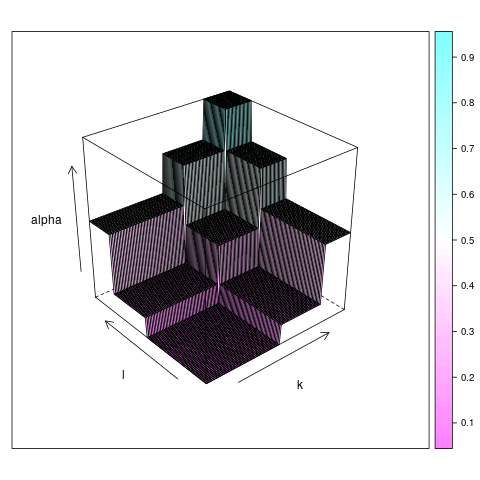
\includegraphics[trim=50 50 50 50, width=.5\textwidth, clip=T]{\fignet/FigGraphon-SBM-graphon-alpha}
    \end{tabular}
  \end{tabular}
  
%   \vspace{-.1\textheight}
  \pause 
  \paragraph{Same representation for all $K$.}
  $
  Y_{ij} | (U_i, U_j) \sim \Pcal\left(\exp(\phi(U_i, U_j) + x_{ij}^\trans \beta \right)
  $
  
  }

%====================================================================
\frame{\frametitle{Tree network residual structure}

%   \vspace{-.2\textheight}
  \hspace{-.04\textwidth}
  \begin{tabular}{cc}
    \begin{tabular}{p{.4\textwidth}}
      \paragraph{Residual graphon.} \\
      Each particle $\theta^m$ provides an estimate of $\phi^m(u, v)$ \\
      ~ \\
      ~ \\
      All estimates can be averaged (over both $m$ and $K$)
    \end{tabular}
    & 
    \pause
%     \hspace{-.05\textwidth}
    \begin{tabular}{p{.5\textwidth}}
    \paragraph{$\widehat{\Esp}\left(\phi(u, v) \mid Y)\right)$:} \\
    \includegraphics[trim=50 100 50 100, width=.5\textwidth]{\figtree/Tree-all-V10-M5000-graphon}
    \end{tabular}
  \end{tabular}
  
%   \vspace{-.1\textheight}
  \pause
  \paragraph{Interpretation.}
  \begin{itemize}
   \item A remaining individual effect (some species interact more than other in average)
   \item A small fraction of species interact much less than expected.
  \end{itemize}

}
  
%====================================================================
\frame{\frametitle{Onager residual structure}

  
  \begin{tabular}{ll}
  \paragraph{$\widehat{\Esp}\left(\phi(u, v) \mid Y)\right)$}
  &
  \paragraph{$\widehat{\Esp}\left((U_i) \mid Y)\right)$}
  \\
  \includegraphics[trim=50 150 50 100, width=.5\textwidth]{\figzebra/WildAss-which-status-V10-M5000-graphon}
  &
  \includegraphics[trim=50 100 50 50, width=.35\textwidth]{\figzebra/WildAss-which-status-V10-M5000-Ui}   
  \end{tabular}

  \bigskip \bigskip \bigskip 
  \paragraph{Interpretation.}
  \begin{itemize}
   \item A remaining individual effect, not related to the sex or the age
  \end{itemize}

}
  
%====================================================================
%====================================================================
\section*{Conclusion}
%====================================================================
\frame{\frametitle{Conclusion} 

  \paragraph{Variational approximations.} 
  \begin{itemize}
   \item Efficient algorithms, reasonably easy to implement 
   \item Good empirical behavior but few theoretical guaranties
  \end{itemize}

  \bigskip \bigskip \pause
  \paragraph{Pragmatic point-of-view:} 
  \begin{itemize}
   \item Use V(B)EM as a first step for regular statistical inference
  \end{itemize}

  \bigskip \bigskip \pause
  \paragraph{Extensions.} 
  \begin{itemize}
   \item Other latent variable models
   \item e.g. Poisson log-normal for the joint analysis of species abundance in ecology
  \end{itemize}


}

%====================================================================
\frame[allowframebreaks]{ \frametitle{References}
  {%\footnotesize
   \tiny
   \bibliography{/home/robin/Biblio/BibGene}
%    \bibliographystyle{/home/robin/LATEX/Biblio/astats}
   \bibliographystyle{alpha}
  }
}

%====================================================================
\backupbegin
%====================================================================

%====================================================================
\backupend
%====================================================================

%====================================================================
%====================================================================
\end{document}
%====================================================================
%====================================================================
  
  \hspace{-.025\textwidth}
  \begin{tabular}{cc}
    \begin{tabular}{p{.5\textwidth}}
    \end{tabular}
    & 
    \hspace{-.02\textwidth}
    \begin{tabular}{p{.5\textwidth}}
    \end{tabular}
  \end{tabular}

